% Options for packages loaded elsewhere
\PassOptionsToPackage{unicode}{hyperref}
\PassOptionsToPackage{hyphens}{url}
%
\documentclass[
  10pt,
  a4paper,
]{article}
\usepackage{amsmath,amssymb}
\usepackage{iftex}
\ifPDFTeX
  \usepackage[T1]{fontenc}
  \usepackage[utf8]{inputenc}
  \usepackage{textcomp} % provide euro and other symbols
\else % if luatex or xetex
  \usepackage{unicode-math} % this also loads fontspec
  \defaultfontfeatures{Scale=MatchLowercase}
  \defaultfontfeatures[\rmfamily]{Ligatures=TeX,Scale=1}
\fi
\usepackage{lmodern}
\ifPDFTeX\else
  % xetex/luatex font selection
  \setmainfont[]{DejaVu Sans}
  \setmonofont[]{DejaVu Sans Mono}
\fi
% Use upquote if available, for straight quotes in verbatim environments
\IfFileExists{upquote.sty}{\usepackage{upquote}}{}
\IfFileExists{microtype.sty}{% use microtype if available
  \usepackage[]{microtype}
  \UseMicrotypeSet[protrusion]{basicmath} % disable protrusion for tt fonts
}{}
\makeatletter
\@ifundefined{KOMAClassName}{% if non-KOMA class
  \IfFileExists{parskip.sty}{%
    \usepackage{parskip}
  }{% else
    \setlength{\parindent}{0pt}
    \setlength{\parskip}{6pt plus 2pt minus 1pt}}
}{% if KOMA class
  \KOMAoptions{parskip=half}}
\makeatother
\usepackage{xcolor}
\usepackage[margin=19mm]{geometry}
\usepackage{longtable,booktabs,array}
\usepackage{calc} % for calculating minipage widths
% Correct order of tables after \paragraph or \subparagraph
\usepackage{etoolbox}
\makeatletter
\patchcmd\longtable{\par}{\if@noskipsec\mbox{}\fi\par}{}{}
\makeatother
% Allow footnotes in longtable head/foot
\IfFileExists{footnotehyper.sty}{\usepackage{footnotehyper}}{\usepackage{footnote}}
\makesavenoteenv{longtable}
\usepackage{graphicx}
\makeatletter
\def\maxwidth{\ifdim\Gin@nat@width>\linewidth\linewidth\else\Gin@nat@width\fi}
\def\maxheight{\ifdim\Gin@nat@height>\textheight\textheight\else\Gin@nat@height\fi}
\makeatother
% Scale images if necessary, so that they will not overflow the page
% margins by default, and it is still possible to overwrite the defaults
% using explicit options in \includegraphics[width, height, ...]{}
\setkeys{Gin}{width=\maxwidth,height=\maxheight,keepaspectratio}
% Set default figure placement to htbp
\makeatletter
\def\fps@figure{htbp}
\makeatother
\setlength{\emergencystretch}{3em} % prevent overfull lines
\providecommand{\tightlist}{%
  \setlength{\itemsep}{0pt}\setlength{\parskip}{0pt}}
\setcounter{secnumdepth}{-\maxdimen} % remove section numbering
\ifLuaTeX
\usepackage[bidi=basic]{babel}
\else
\usepackage[bidi=default]{babel}
\fi
\babelprovide[main,import]{french}
\ifPDFTeX
\else
\babelfont{rm}[]{DejaVu Sans}
\fi
% get rid of language-specific shorthands (see #6817):
\let\LanguageShortHands\languageshorthands
\def\languageshorthands#1{}
\usepackage{etoolbox}
\usepackage{microtype}
\usepackage{float}
\floatplacement{figure}{H}
\sloppy
\setlength{\emergencystretch}{5em}
\AtBeginEnvironment{longtable}{\small}
\ifLuaTeX
  \usepackage{selnolig}  % disable illegal ligatures
\fi
\IfFileExists{bookmark.sty}{\usepackage{bookmark}}{\usepackage{hyperref}}
\IfFileExists{xurl.sty}{\usepackage{xurl}}{} % add URL line breaks if available
\urlstyle{same}
\hypersetup{
  pdftitle={Transport positif, réserve et brique initiale},
  pdfauthor={Vincent P. P. NOËL - dossier de recherche, rédaction assistée},
  pdflang={fr-FR},
  hidelinks,
  pdfcreator={LaTeX via pandoc}}

\title{Transport positif, réserve et brique initiale}
\usepackage{etoolbox}
\makeatletter
\providecommand{\subtitle}[1]{% add subtitle to \maketitle
  \apptocmd{\@title}{\par {\large #1 \par}}{}{}
}
\makeatother
\subtitle{Document 78 - Continuer vers le signe global de Weil}
\author{Vincent P. P. NOËL - dossier de recherche, rédaction assistée}
\date{14 octobre 2026}

\begin{document}
\maketitle

{
\setcounter{tocdepth}{2}
\tableofcontents
}
\hypertarget{ce-que-cette-passe-apporte}{%
\section{Ce que cette passe apporte}\label{ce-que-cette-passe-apporte}}

Une contribution première devient une demande de masse située en un
point. La partie archimédienne fournit une matière continue. Un
appariement positif qui conserve le centre moyen de chaque demande
impose le signe par convexité. Le problème est de construire cet
appariement pour \textbf{toutes} les demandes.

Nous avons maintenant trois briques avec leurs preuves : une sommation
de lignes compatible avec une réserve infinie ; un bilan qui relie le
stock au point zéro aux défauts de Fenchel ; une opération initiale non
minimale qui consomme entièrement ce stock et laisse intacte
l'obligation globale suivante. Les calculs finis et la confrontation
indépendante accompagnent ces briques.

\textbf{Aucun signe global n'est démontré.} Un balayage qui réussirait à
tous les rangs serait équivalent à RH. La construction initiale
ci-dessous est, elle, établie sans RH dans le modèle d'intervalles
déclaré.

\begin{figure}
\centering
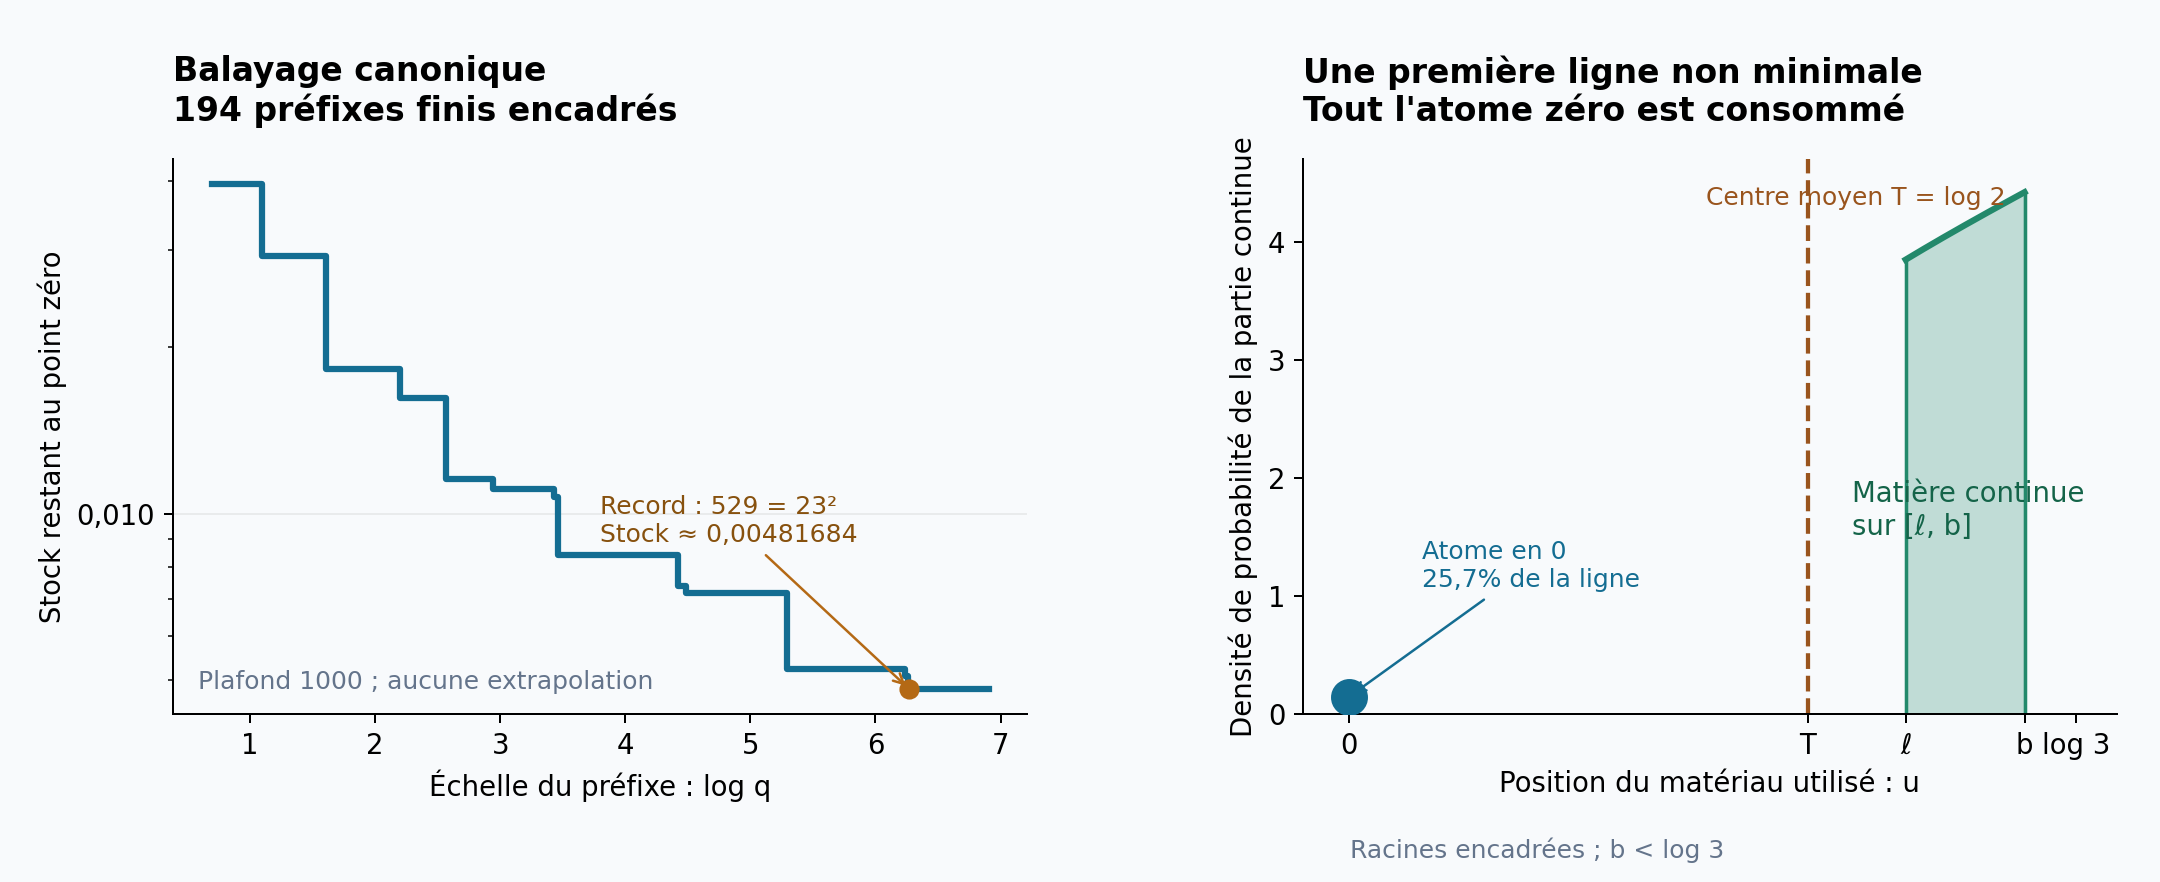
\includegraphics{78_CARTE_TRANSPORT.png}
\caption{Le stock du balayage canonique et une autre façon de traiter la
première ligne.}
\end{figure}

\hypertarget{les-objets-dans-un-ordre-lisible}{%
\section{1. Les objets, dans un ordre
lisible}\label{les-objets-dans-un-ordre-lisible}}

Le paramètre \(t\) désigne une échelle logarithmique. Il ne désigne pas
l'abscisse d'un zéro. Pour une puissance première \(q=p^k\), poser

\[
x_q=\log q,\qquad c_q=\frac{\log p}{\sqrt q}.
\]

Le signal arithmétique de Suzuki s'écrit

\[
S(t)=A(t)-\sum_{q=p^k}c_q(t-x_q)_+,\qquad t\ge0,
\]

\[
\begin{aligned}
A(t)&=4(e^{t/2}+e^{-t/2}-2)-\frac{C_0t}{2}
       +\sum_{n\ge0}\frac{1-e^{-b_nt}}{b_n^2},\\
C_0&=\log(8\pi)+\gamma_E+\frac{\pi}{2},
\qquad b_n=2n+\frac12.
\end{aligned}
\]

Le symbole \((z)_+\) signifie \(\max(z,0)\). Pour une mesure positive
\(\lambda\), son potentiel est

\[
\mathcal P_\lambda(t)=\int(t-u)_+\,\lambda(du).
\]

Les théorèmes 1.6 et 1.7 de Suzuki2023 donnent, pour ce signal précis,
\(RH\iff S\ge0\) partout et \(RH\iff S\) bornée. Son extension2025
permet de demander seulement un signe après un seuil. Ce pont utilise la
transformée liée à \(\xi'/\xi\) et l'absence de zéros réels de la
fonction complétée. Un signal positif quelconque ne possède pas ce
pouvoir.

Fixons \(T=\log2\). Une différentiation exacte donne

\[
\begin{aligned}
A'(t)&=2(e^{t/2}-e^{-t/2})-\frac{C_0}{2}
       +\operatorname{atanh}(e^{-t/2})+\arctan(e^{-t/2}),\\
\beta(t)&=A''(t)=e^{t/2}
                 -\frac{e^{-5t/2}}{1-e^{-2t}}>0\quad(t\ge T).
\end{aligned}
\]

Poser \(m=S(T)/T\) et \(a=S'(T+)\), la dérivée droite incluant \(q=2\).
Les encadrements donnent \(m>0\), \(a<0\). Ici les mesures se
simplifient en

\[
\mu=m\delta_0+\mathbf1_{(T,\infty)}\beta(u)\,du,\qquad
\nu=(m-a)\delta_T+\sum_{q>2}c_q\delta_{x_q}.
\]

Elles sont positives, localement finies, de masse totale infinie. On a
\(\mathcal P_\mu-\mathcal P_\nu=S\) pour \(t\ge T\), et \(mt\) pour
\(0\le t<T\). Le raccord \((m-a)\delta_T\) a une masse d'environ
\(0{,}35684525\) ; ce n'est pas la masse première \(c_2\), d'environ
\(0{,}49012907\).

Les unités fictives peuvent rendre le bilan lisible : si \([t]=L\) et
\([S]=E\), les masses \(c,m\) ont l'unité \(E/L\), le premier moment
l'unité \(E\), et la densité \(\beta\) l'unité \(E/L^2\). Cette
convention ne crée aucun signe.

\hypertarget{brique-a-des-lignes-fixuxe9es-une-fois-pour-toutes}{%
\section{2. Brique A : des lignes fixées une fois pour
toutes}\label{brique-a-des-lignes-fixuxe9es-une-fois-pour-toutes}}

Écrire \(\nu=\sum_jc_j\delta_{x_j}\). Supposons que l'on construise des
mesures positives \(\eta_j\) telles que

\[
\eta_j(\mathbb R)=c_j,\qquad
\int u\,\eta_j(du)=c_jx_j,\qquad
\sum_{j\le N}\eta_j\le\mu\quad\text{pour tout }N.
\]

Alors \(\sigma=\sum_j\eta_j\le\mu\) est une mesure bien définie. Chaque
\(K_{x_j}=\eta_j/c_j\) est un noyau de probabilité de barycentre
\(x_j\). Par Jensen et sommation de quantités non négatives,

\[
\mathcal P_\mu(t)-\mathcal P_\nu(t)
\ge\sum_j\left[\mathcal P_{\eta_j}(t)-c_j(t-x_j)_+\right]\ge0.
\]

À \(t\) fixé, les deux potentiels sont finis : aucune soustraction de
masses globales infinies n'est faite. Fixer les lignes successivement
évite la fuite de premier moment qui peut survenir dans une limite de
plans recalculés.

\textbf{Coup double conditionnel.} Ce sous-couplage suffirait au signe,
donc à RH. Il couvrirait ensuite automatiquement toute \(\mu\). En
effet, son résidu \(\rho=\mu-\sigma\ge0\) vérifie
\(\mathcal P_\rho\le S\). Une masse positive de \(\rho\) dans \([0,B]\)
entraînerait \(S(t)\ge(t-B)\rho([0,B])\), contrairement à la bornitude
sous RH.

\hypertarget{brique-b-un-geste-de-transport-et-son-vrai-test}{%
\section{3. Brique B : un geste de transport et son vrai
test}\label{brique-b-un-geste-de-transport-et-son-vrai-test}}

Pour un reliquat positif \(R\) de masse infinie, notons \(G_R(v)\) son
quantile : on compte la matière depuis la gauche et l'on lit la position
de la \(v\)-ième unité de masse.

Pour une demande \(c\delta_x\), un bloc de masse \(c\) existe si et
seulement si

\[
\frac1c\int_0^cG_R(v)\,dv\le x.
\tag{A}
\]

Si (A) est satisfaite, on translate le bloc de masse jusqu'à trouver
\(s\ge0\) tel que

\[
\frac1c\int_s^{s+c}G_R(v)\,dv=x,\qquad
\eta=(G_R)_\#\bigl(\mathbf1_{[s,s+c]}dv\bigr).
\]

La moyenne du bloc est continue, non décroissante et tend vers l'infini.
Sa valeur initiale est la plus petite moyenne possible pour une
sous-mesure de masse \(c\). Cela prouve le critère et la conservation.
On retire \(\eta\) de \(R\), puis l'on traite la demande suivante.

La positivité du reliquat est automatique après un retrait admissible.
\textbf{L'admissibilité de la prochaine ligne ne l'est pas.} La théorie
finie des ombres et leur associativité, après troncature suffisamment
grande, montrent que la réussite à tous les rangs équivaut à
\(\mathcal P_\nu\le\mathcal P_\mu\) partout. Le test infini reste donc
exactement l'obligation de RH.

\hypertarget{brique-c-le-stock-est-un-duxe9faut-arithmuxe9tique}{%
\section{4. Brique C : le stock est un défaut
arithmétique}\label{brique-c-le-stock-est-un-duxe9faut-arithmuxe9tique}}

Soit \(S_N=\mathcal P_\mu-\mathcal P_{\nu_N}\), où le préfixe inclut le
raccord en \(T\). Pour le balayage canonique réussi, le stock restant à
zéro vaut

\[
r_N=(\mu-\sigma_N)\{0\}=\inf_{t>0}\frac{S_N(t)}t.
\tag{B}
\]

\textbf{Preuve élémentaire.} Jensen donne \(S_N(t)\ge r_Nt\).
Considérons la dernière ligne ayant pris de la matière en zéro, et son
extrémité droite \(b\). Elle épuise tout le reliquat entre zéro et
\(b\), sauf \(r_N\delta_0\). Les lignes précédentes ont leur extrémité
droite au plus \(b\) : sinon une ligne antérieure aurait un barycentre
supérieur à celui de cette ligne, car les intervalles déjà balayés ne
contiennent plus de matière disponible. Les lignes suivantes qui évitent
zéro prennent leur masse au-delà de \(b\). Au point \(b\), tous les
écarts de Jensen concernés sont donc nuls : \(S_N(b)=r_Nb\). Si aucune
ligne ne prend en zéro, le rapport vaut \(m\) avant le premier support
positif.

Ordonner les puissances premières originales, y compris \(q=2\), et
poser

\[
C_j=\sum_{i\le j}c_i,\qquad L_j=\sum_{i\le j}c_ix_i.
\]

La somme des charnières est le maximum des droites \(C_jt-L_j\). Ainsi,
indépendamment de l'existence d'un transport, le budget radial du
préfixe est

\[
\widehat r_N=\min\{m,d_1,\ldots,d_N\},\qquad
d_j=\min_{t\ge T}\frac{A(t)-C_jt+L_j}{t}.
\tag{C}
\]

Pour les préfixes non vides de ce dossier, l'optimum est intérieur. Son
point \(\tau_j\) et sa valeur satisfont

\[
\tau_jA'(\tau_j)-A(\tau_j)=L_j,\qquad
d_j=A'(\tau_j)-C_j.
\]

L'équation est strictement croissante puisque sa dérivée vaut
\(t\beta(t)>0\). Le terme linéaire contenant \(C_0\) s'y annule
exactement.

Le lien avec le défaut de Fenchel \(H_j=L_j-A_T^*(C_j)\) est précis. Ici
\(A_T^*(c)=\sup_{t\ge T}(ct-A(t))\). Si \(A'(\theta_j)=C_j\), alors

\[
H_j=\int_{\theta_j}^{\tau_j}u\beta(u)\,du,\qquad
d_j=\int_{\theta_j}^{\tau_j}\beta(u)\,du.
\tag{D}
\]

Ils ont exactement le même signe. Le défaut de Fenchel devient donc un
stock de transport, et réciproquement. Si le transport existe, (B) et
(C) coïncident. La nonnégativité de tous les \(\widehat r_N\) reste à
démontrer.

\hypertarget{la-bifurcation-traiter-toute-lorigine-en-une-fois}{%
\section{5. La bifurcation : traiter toute l'origine en une
fois}\label{la-bifurcation-traiter-toute-lorigine-en-une-fois}}

Le balayage minimal laisse \(r_N>0\) après tout préfixe fini sous RH,
alors que son stock final doit être nul. Il lui faut donc une infinité
de lignes issues de positions arbitrairement grandes qui alimentent
encore zéro. \textbf{Ce balayage précis a nécessairement une portée non
bornée.} Cela ne s'applique pas à tous les noyaux possibles.

Une autre première ligne élimine ce stock immédiatement. Construire

\[
\eta=m\delta_0+\mathbf1_{[\ell,b]}\beta(u)\,du,
\]

avec

\[
\int_\ell^b\beta(u)\,du=-a,\qquad
\int_\ell^bu\beta(u)\,du=T(m-a).
\tag{E}
\]

Elle a la masse \(m-a\) et le barycentre \(T\). De plus \(\eta\le\mu\).
Le calcul par intervalles établit l'existence d'un couple exact tel que

\[
0{,}84097046\le\ell\le0{,}84097048,\qquad
1{,}02059031<b<1{,}02059034<\log3.
\]

\textbf{Justification de l'existence.} Pour chaque \(\ell\), l'équation
de masse détermine un unique \(b(\ell)\), car \(\beta>0\). À masse
fixée, la dérivée du premier moment par rapport à \(\ell\) est
\((b-\ell)\beta(\ell)>0\). Les deux bornes rationnelles de \(\ell\)
donnent des écarts de moment de signes opposés, encadrés strictement. Le
théorème des valeurs intermédiaires donne le couple exact de (E). Les
décimales ne sont pas utilisées comme des coefficients exacts du noyau.

Poser \(c=m-a\) et \(J=\mathcal P_\eta-c(t-T)_+\ge0\). Puisque toute la
ligne est supportée dans \([0,b]\), son écart \(J\) est nul pour
\(t\ge b\). Le nouveau problème porte sur

\[
\mu'=\mu-\eta,\qquad \nu'=\nu-c\delta_T.
\]

Son signal \(\mathcal P_{\mu'}-\mathcal P_{\nu'}\) est automatiquement
non négatif avant \(\log3\), car aucun atome de \(\nu'\) n'y intervient,
et il égale exactement \(S\) dès \(b\). L'obligation globale est
conservée.

\textbf{Deux effets acquis sans RH :} toute la réserve en zéro est
consommée ; la première demande est satisfaite par une seule ligne de
portée \(T\). Il faut recalculer les lignes suivantes sur \(\mu'\). Les
anciennes lignes du balayage minimal ne peuvent pas être recopiées sans
contrôle.

\hypertarget{ce-que-les-calculs-finis-uxe9tablissent}{%
\section{6. Ce que les calculs finis
établissent}\label{ce-que-les-calculs-finis-uxe9tablissent}}

Le plafond \(q\le1000\) contient 193 puissances premières originales. Le
transport utilise 192 atomes \(q>2\) et un raccord en \(T\). Le fichier
de réserve encadre 194 préfixes, préfixe vide compris.

\begin{longtable}[]{@{}
  >{\raggedright\arraybackslash}p{(\columnwidth - 4\tabcolsep) * \real{0.3333}}
  >{\raggedright\arraybackslash}p{(\columnwidth - 4\tabcolsep) * \real{0.3333}}
  >{\raggedright\arraybackslash}p{(\columnwidth - 4\tabcolsep) * \real{0.3333}}@{}}
\toprule\noalign{}
\begin{minipage}[b]{\linewidth}\raggedright
Objet
\end{minipage} & \begin{minipage}[b]{\linewidth}\raggedright
Résultat
\end{minipage} & \begin{minipage}[b]{\linewidth}\raggedright
Portée
\end{minipage} \\
\midrule\noalign{}
\endhead
\bottomrule\noalign{}
\endlastfoot
Réserve radiale minimale & Environ \(0{,}00481683660325\), record
\(q=529=23^2\) & Préfixes finis, intervalles 400 bits \\
Position du record & Environ \(6{,}2777323555\) & Minimum du signal
tronqué divisé par \(t\) \\
Noyaux continus explicites & Balayage à 60 chiffres, bilans exportés &
Diagnostic, sans encadrement de chaque noyau \\
Première ligne non minimale & Racines de (E) encadrées, \(\eta\le\mu\) &
Brique initiale sans RH \\
Signe scalaire original & Fenêtre \([\log2,\log1000]\) couverte & Ne
couvre pas la queue ni toutes les formes de Weil \\
\end{longtable}

La variante non minimale a été recalculée sur les trois plafonds
suivants. Les largeurs sont celles des supports des noyaux, hors ligne
artificielle de bord.

\begin{longtable}[]{@{}
  >{\raggedleft\arraybackslash}p{(\columnwidth - 4\tabcolsep) * \real{0.3333}}
  >{\raggedleft\arraybackslash}p{(\columnwidth - 4\tabcolsep) * \real{0.3333}}
  >{\raggedleft\arraybackslash}p{(\columnwidth - 4\tabcolsep) * \real{0.3333}}@{}}
\toprule\noalign{}
\begin{minipage}[b]{\linewidth}\raggedleft
Plafond
\end{minipage} & \begin{minipage}[b]{\linewidth}\raggedleft
Largeur maximale canonique
\end{minipage} & \begin{minipage}[b]{\linewidth}\raggedleft
Largeur maximale après la nouvelle première ligne
\end{minipage} \\
\midrule\noalign{}
\endhead
\bottomrule\noalign{}
\endlastfoot
10 & 2,275156 & 1,564702 \\
100 & 4,515697 & 3,815500 \\
1000 & 6,277732 & 5,580028 \\
\end{longtable}

La réserve en zéro est nulle aux trois plafonds ; les préfixes communs
de la variante concordent dans les fichiers à 60 chiffres. Il reste à
1000 une réserve \textbf{diffuse} d'environ \(0{,}0054169160\) près de
\(T\). Le coût quadratique total du plan fermé est inchangé : les
marginales le déterminent. Le retrait de l'atome initial ne paie donc
pas toute la difficulté globale. Ces comparaisons restent des
diagnostics.

Une fermeture finie permet aussi de vérifier les bilans au bord. Pour
\(L=\log X\), choisir \(U>L\) tel que

\[
\int_L^U(u-L)\beta(u)\,du=S_X(L),
\qquad D=S_X'(U)\ge0.
\]

Les mesures \(\mu|_{[0,U]}\) et \(\nu_X+D\delta_L\) ont alors mêmes
masse et premier moment. Après \(L\), leur différence de potentiels vaut
\(\int_t^U(u-t)\beta(u)\,du\), puis zéro après \(U\). À \(X=1000\),
\(U\) est environ \(6{,}9666484578\), et \(D\) environ
\(1{,}9417621728\).

\textbf{Le bord \(D\delta_L\) est artificiel.} Il ne peut pas
représenter littéralement une combinaison positive de futurs atomes
situés strictement après \(L\) : à masse \(D\) égale, leur moment serait
strictement supérieur à \(DL\). Il faut rouvrir ce bord et ajouter la
nouvelle matière continue.

\hypertarget{ce-que-laudit-ferme-et-ce-quil-laisse-ouvert}{%
\section{7. Ce que l'audit ferme, et ce qu'il laisse
ouvert}\label{ce-que-laudit-ferme-et-ce-quil-laisse-ouvert}}

Un noyau entièrement atomique ne peut fournir la densité \(\beta\,du\).
Une loi fixe de déplacement, centrée et de portée bornée, est également
impossible : le théorème des nombres premiers imposerait
\(\int e^{-z/2}k(dz)=1\), tandis que Jensen strict impose alors
\(k=\delta_0\), incompatible avec une cible diffuse.

Une portée bornée pour des noyaux \textbf{variables et non minimaux}
n'est pas exclue ici. En revanche, elle ne peut accompagner une variance
uniformément positive : la bornitude du signal sous RH impose une
variance moyenne pondérée qui tend vers zéro à grande échelle.

La brique initiale ne fournit pas le signe du résidu à toutes les
échelles. Les prochaines questions sont maintenant concrètes :

\begin{enumerate}
\def\labelenumi{\arabic{enumi}.}
\tightlist
\item
  Construire une règle non minimale pour les demandes suivantes, en
  conservant exactement leurs masses et leurs moments.
\item
  Trouver un invariant arithmétique qui impose l'admissibilité de chaque
  ajout, sans supposer une borne sur les premiers déjà équivalente à RH.
\item
  Conserver les lignes déjà validées et payer explicitement le nouveau
  bord.
\item
  Obtenir toutes les échelles, sans marge positive uniforme : sous RH,
  le signal a un infimum nul au-delà de tout seuil.
\end{enumerate}

La couverture logique est acquise pour une construction de toutes les
lignes. La \textbf{loi de signe arithmétique globale} reste le verrou.
Ces briques donnent un sens opératoire au transport ; elles ne
remplacent pas sa preuve globale.

\newpage

\hypertarget{sources-statut-et-reproduction}{%
\section{Sources, statut et
reproduction}\label{sources-statut-et-reproduction}}

Les critères de Suzuki et la théorie finie des ombres sont des résultats
publiés. Les bilans, preuves auxiliaires, encadrements et variantes de
ce document constituent un dossier de travail non relu extérieurement.
Aucune priorité de découverte n'est revendiquée.

\begin{itemize}
\tightlist
\item
  M. Suzuki, \emph{Aspects of the screw function corresponding to the
  Riemann zeta-function}, JLMS108 (2023), 1448-1487, théorèmes 1.6 et
  1.7 : \url{https://arxiv.org/pdf/2206.03682}.
\item
  M. Suzuki, \emph{Screw functions of Dirichlet series in the extended
  Selberg class}, version2025, théorème 1.1 :
  \url{https://arxiv.org/pdf/2209.12832}.
\item
  M. Beiglböck et N. Juillet, \emph{On a problem of optimal transport
  under marginal martingale constraints}, Ann. Probab.44 (2016), 42-106,
  ombre d'un atome et associativité :
  \url{https://www.mat.univie.ac.at/~mathias/BJ_AOP.pdf}.
\item
  M. Beiglböck, D. Hobson et D. Norgilas, \emph{The potential of the
  shadow measure} (2020), théorèmes 2 et 3, lecture complémentaire :
  \url{https://arxiv.org/pdf/2008.09936}.
\end{itemize}

Avec mpmath1.3.0 et le mini-corpus fourni :

\begin{verbatim}
python3 initial_block_certificate.py --corpus mini_corpus \
    --output bloc_initial_certificat.json
python3 radial_reserve.py --corpus mini_corpus --cutoff 1000 \
    --output reserve_radiale_1000.json
python3 exploration/shadow_sweep_high_precision.py 1000
\end{verbatim}

Le dossier exploration contient aussi la variante
nonminimal\_shadow\_sweep.py et sa comparaison aux plafonds 10, 100 et
1000.

Les solveurs approchés proposent les positions. Les deux premiers
scripts contrôlent les signes par intervalles, avec encadrement d'Euler
et queue exponentielle géométrique. Le dernier fournit un diagnostic de
noyaux à 60 chiffres. Aucun programme n'utilise de zéros de \(\zeta\).

\end{document}
